\chapter{Projet}

\section{Présentation du projet}
Afin d'étudier le framework, j'ai décidé de créer une application web pour le mettre en oeuvre et mieux comprendre les mécanismes de fonctionnement. Cette étude portant sur Angular la partie back-end ne sera pas étudiée dans ce rapport.
\subsection{Sujet Labo}
L'application utilisée pour étudier le framework Angular est une application d'enregistrement de facture. Cette application ne gère pas la création du document contractuel en lui même, mais simplement la configuration de la facture pour pouvoir mettre en oeuvre l'utilisation des composants web. La création du document pourrait facilement être générée grâce à une librairie tierce telle que \texttt{jsPDF}\cite{github:jsPDF}. Nous pouvons donc créer des clients, créer des produits et créer des factures auxquelles on attribue un client et un ou des produits. Le montant de la facture est ainsi calculé en fonction des produits et de leurs quantités.
\subsection{Back-end}

Même si nous ne nous concentrerons pas sur la partie back-end dans ce rapport, certaines fonctions comme la protection du routage nécessitent l'utilisation de fonctions serveur comme l'authentification par exemple. Pour cela, j'utilise la solution Firebase de Google qui permet l'utilisation de son API pour mettre en place différents services comme la gestion d'authentification ou encore une base de données NoSQL\footnote{Firebase : https://firebase.google.com/}

\section{ANGULAR}
\subsection{Les composants}
Les composants sont le coeur du fonctionnement d'Angular. En effet, chaque élément fonctionnel peut être décomposé en composant web. Dans notre application, comme on peut le voir a la figure \ref{composant-app}, chaque élément encordé par des pointillés représente une instance d'un composant.
\begin{figure}[h]
	\centering
	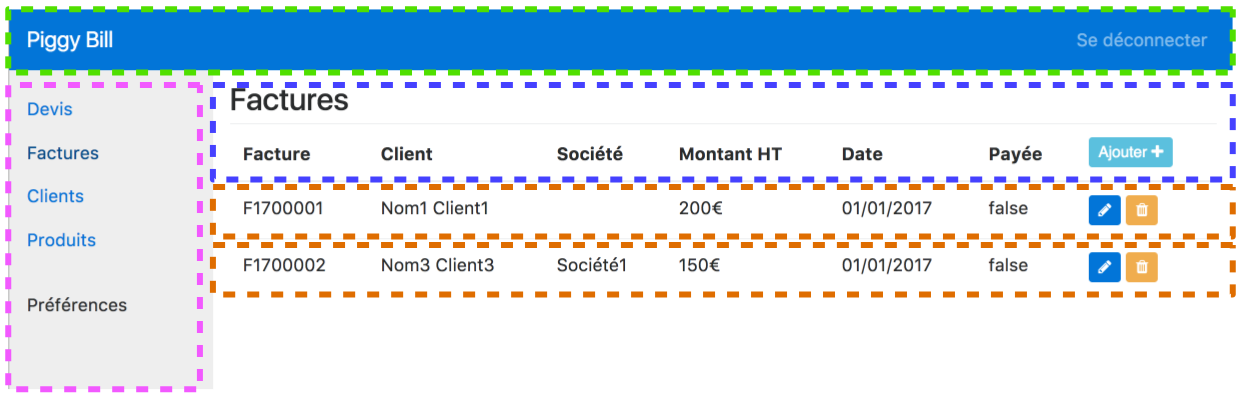
\includegraphics[width=16.8cm]{composants-application}
	\caption{Exemple de composant dans l'application}
	\label{composant-app}
\end{figure}
\subsubsection{Description}
Nous allons voir de quoi est composé un composant. Pour rappel, la commande pour générer un composant en utilisant le CLI est :
\begin{lstlisting}[language=bash]
ng generate component mon-nouveau-composant
\end{lstlisting}
Cette commande créer les fichiers suivants :
\begin{figure}[h]
	\centering
	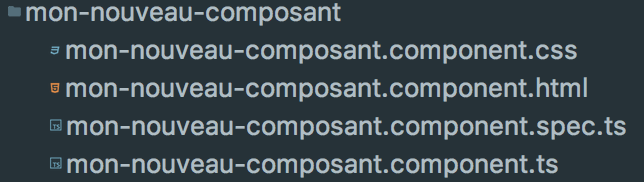
\includegraphics[scale=0.6]{new-component}
	\caption{Structure de fichier d'un composant}
	\label{new-component}
\end{figure}


Le premier fichier, \texttt{mon-nouveau-composant.component.css} contient la feuille de style propre au composant.

\texttt{mon-nouveau-composant.component.html}, contient le template du composant, c'est-à-dire le code HTML qui sera exécuté à chacun des appelles de celui-ci. 

Le fichier \texttt{mon-nouveau-composant.component.spec.ts} est un fichier TypeScript destiné aux tests unitaires du composant. 

Enfin, le fichier \texttt{mon-nouveau-composant.component.ts} est le fichier maître du composant, il déclare et contient les méthodes et la logique du composant. Sur ses quatre fichiers, il est possible de n'utiliser que ce dernier. En effet en ajoutant les commandes \texttt{-inline-template} et \texttt{-inline-style}\cite{angluarcli:doc} on a la possibilité d'intégrer le template HTML et la feuille de style dans le fichier. Cette mise en oeuvre peut être pratique pour les petits composants, car nous n'avons qu'un seul fichier à gérer.

Attardons-nous sur le fichier \texttt{mon-nouveau-composant.component.ts} voici ce qu'il contient à sa création :

\begin{lstlisting}[style=htmlcssjs, caption={mon-nouveau-composant.component.ts}, label=composant]
import { Component, OnInit } from '@angular/core';

@Component({
  selector: 'app-mon-nouveau-composant',
  templateUrl: './mon-nouveau-composant.component.html',
  styleUrls: ['./mon-nouveau-composant.component.css']
})
export class MonNouveauComposantComponent implements OnInit {

  constructor() { }

  ngOnInit() {
  }

}
\end{lstlisting}

Le fichier commence par les imports des classes nécessaires au fonctionnement de notre application. Ici, le composant étant extrêmement basique, on importe uniquement la classe \texttt{Component} pour pouvoir le déclarer en tant que tel, ainsi que la classe \texttt{OnInit} dont je vous décrirais l'utilité plus tard.

\texttt{@Component} est un déporteur qui permet de configurer le composant pour qu'il soit compris par Angular. Ce décorateur attend un objet comprenant les propriétés de configuration de composant. 

\texttt{selector} indique à Angular ce qu’il faudra chercher dans nos pages HTML. À chaque fois que le sélecteur défini sera trouvé dans notre HTML, Angular remplacera l’élément sélectionné par notre composant. Dans notre cas, si dans une page HTML est présent le code \texttt{<app-mon-nouveau-composant></app-mon-nouveau-composant>}, Angular créera une nouvelle instance de notre composant.

Le paramètre \texttt{templateUrl} indique le nom du fichier où se trouve le template HTML pour le composant. Dans le cas de l'utilisation de l'option \texttt{-inline-template} ce paramètre est remplacé par \texttt{template} qui se présente comme suit :

\begin{lstlisting}[style=htmlcssjs, caption={inline-template}]
template: '
	<h1>Code du template</h1>
	<p>Lorem ipsum</p>
'
\end{lstlisting}

Enfin, le paramètre \texttt{styleUrls} a une fonction équivalente que pour le template à la différence qu'ici on utilise un tableau en paramètre pour avoir la possibilité d'utiliser plusieurs feuilles de style pour un seul composant. En utilisant l'option \texttt{-inline-style} on peut également intégrer la feuille de style directement dans le code du composant.

Enfin nous avons la déclaration de la classe \texttt{MonNouveauComposantComponent} qui hérite de la classe abstraite \texttt{OnInit} qui implique la mise en place de la méthode \texttt{ngOnInit()}. Par défaut, le CLI ajoute le constructeur à la classe.

Pour ensuite afficher le composant dans notre application, il suffira d'appeler la balise HTMl correspondante au \texttt{selector} définit, par exemple, pour l'extrait \label{composant}, la balise devra être \texttt{<app-mon-nouveau-composant></app-mon-nouveau-composant>}.

\paragraph{ngOnInit(), ça sert a quoi ?}

La méthode \texttt{ngOnInit()} est appelée par l'implémentation de la classe \texttt{OnInit}, qui fait partie d'un groupe de méthodes qui réagissent en fonction du cycle de vie du composant. Une notion à bien comprendre est que les entrées d'un composant ne sont pas initialisées dans son constructeur, c'est pour cela que l'on utilise les méthodes suivantes :

\begin{itemize}
	\item \texttt{ngOnChanges()} sera la première méthode appelé lorsque qu'une propriété "bindée" aura été modifiée.
	\item \texttt{ngOnInit()} sera appelée une seule fois après le premier changement (alors que \texttt{ngOnChange} est appelée à chaque changement). Cela en fait la phase parfaite pour du travail d’initialisation, comme son nom le laisse à penser. C'est pour cela qu'elle est ajoutée par défaut par le CLI.
	\item \texttt{ngOnDestroy()} est la méthode qui est appelée quand le composant est supprimé du DOM. Cela peut être utilisé pour fermé des connections par exemple.
\end{itemize}

\subsection{DataBinding}

Le data-binding est une des méthodes faire évoluer dynamique le contenu du DOM, il peut permet notamment de passer des données au template HTML ou encore de réagir à des interactions de l'utilisateur. Voici un schéma pour illustrer.
\begin{figure}[h]
	\centering
	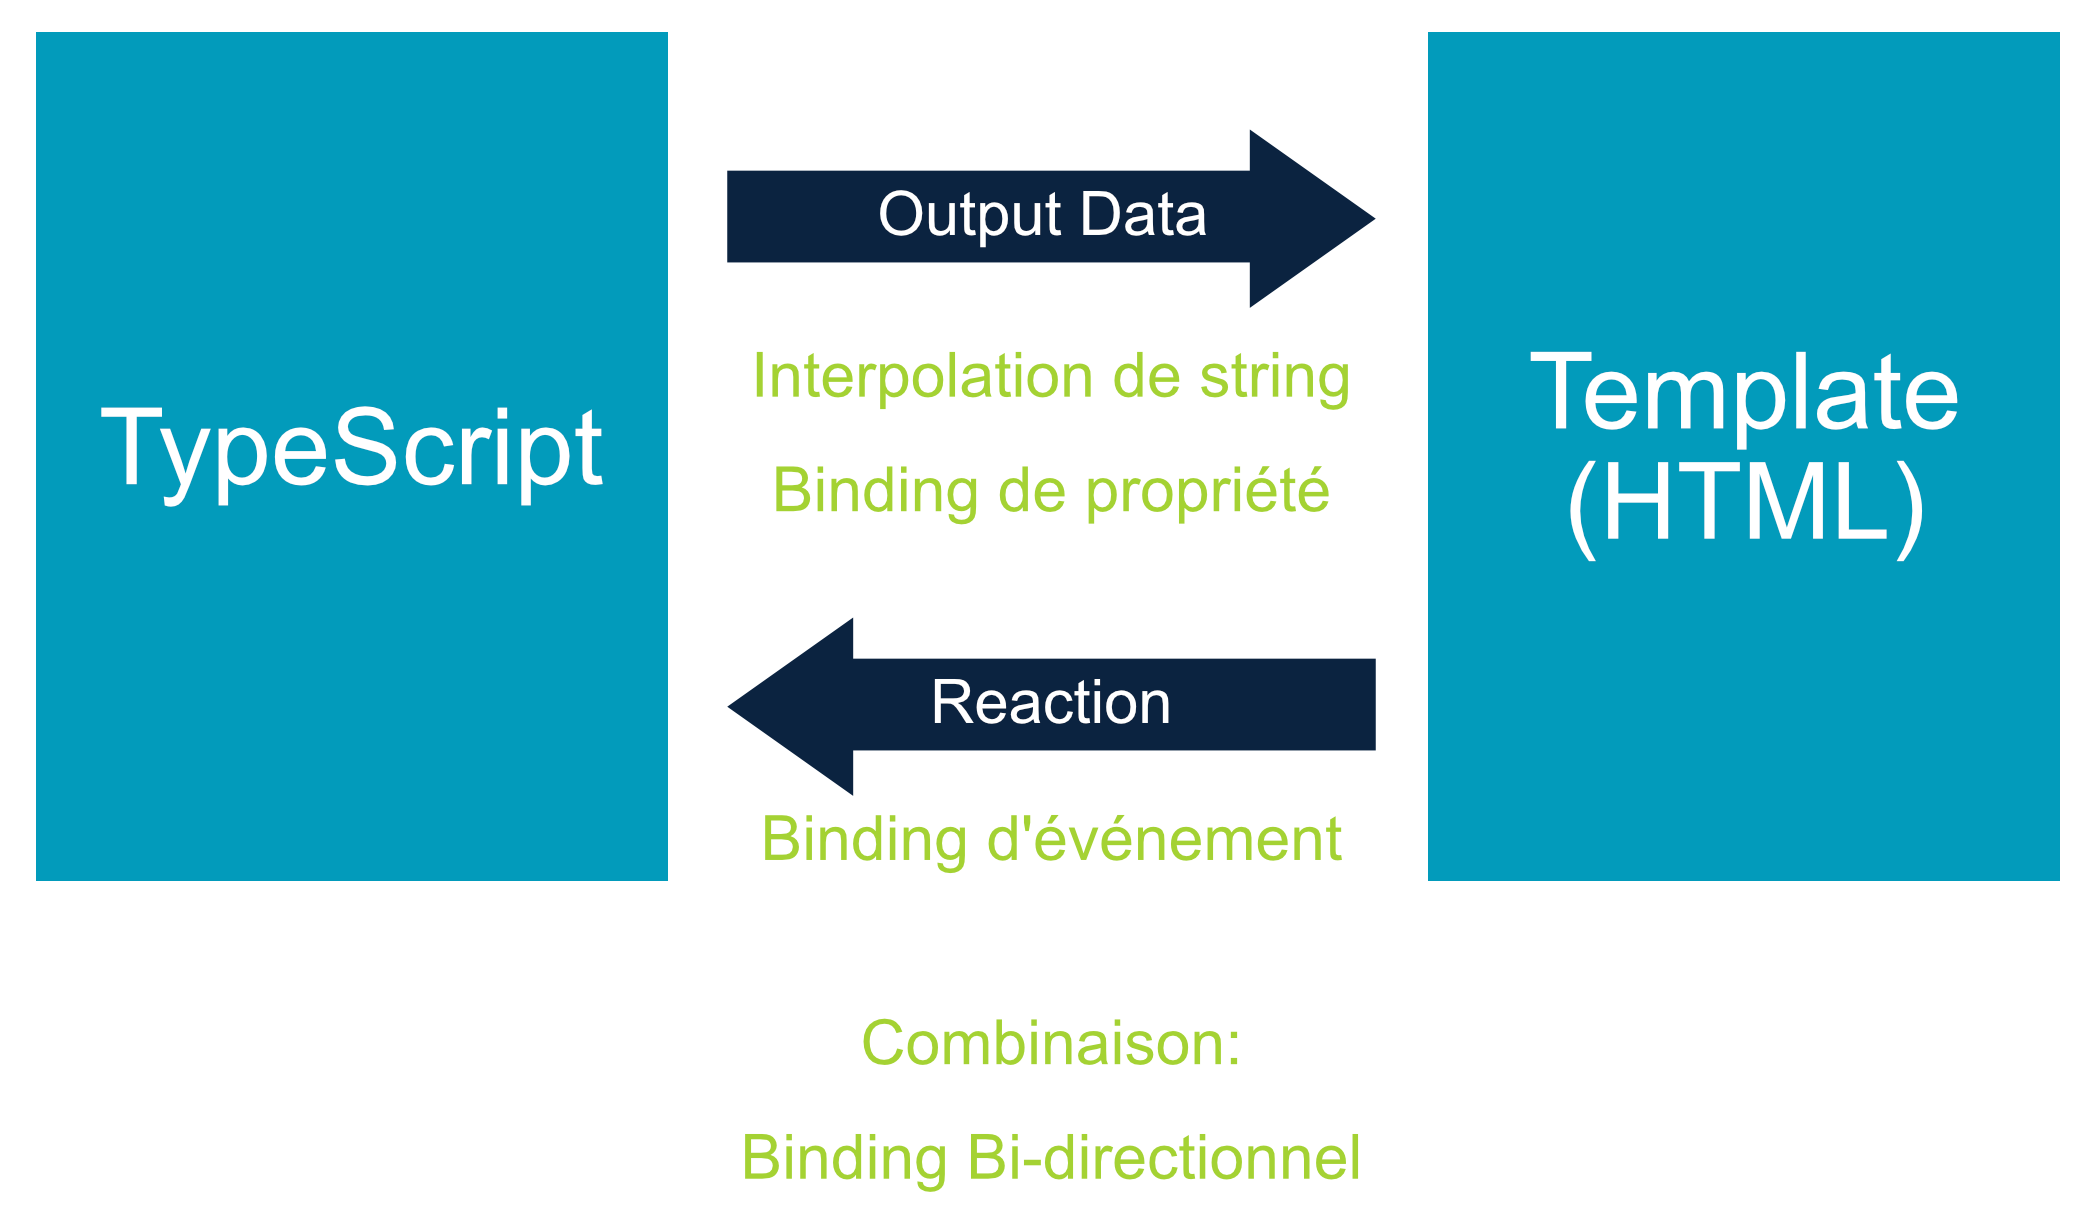
\includegraphics[width=16.8cm]{data-binding}
	\caption{Concept de Databinding}
	\label{databinding}
\end{figure}

\subsubsection{Interpolation de string}
L'interpolation de string permet d'injecter des propriétés d'un composant dans le template HTML en tant que string. Pour cela on utilise la syntaxe avec une double accolade \texttt{\{\{...\}\}}. Dans celle-ci on indiquera soit le non d'une variable que l'on souhaite afficher ou une méthode qui renvoie un string. Les nombres seront convertis pour être affichés. Voici quelques exemples tirés de l'application.

\begin{lstlisting}[style=htmlcssjs, caption={Interpolation de string}, label=stringInt]
<div class="card-block">
	<h4 class="card-title">{{product.designation}}</h4>
	<p class="card-text">Type : {{product.productType}}</p>
	<p class="card-text">Prix HT : {{product.priceExTax}} Euros</p>
    ...
</div>
\end{lstlisting}
Ici, on a déclaré un objet de type \texttt{Product} nommé \texttt{product} dans notre fichier TypeScript du composant. Dans l'extrait de code \ref{stringInt}, on affiche les propriétés \texttt{designation}, \texttt{productType} et \texttt{priceExTax} dans notre template HTML.

\begin{lstlisting}[style=htmlcssjs, caption={Interpolation de string par une méthode}, label=stringIntMeth]
<div class="form-group col-md-2" formGroupName="{{i}}">
	<label for="price">Price HT</label>
	<p id="price">{{getArticlePrice(i)}}</p>
</div>
\end{lstlisting}
Dans cet exemple, on fait appel à une méthode \texttt{getArticlePrice()} pour afficher les informations sur le prix d'un article, \texttt{i} étant l'index de l'article.

L'interpolation de string est donc la méthode à utiliser pour afficher des données dynamiques dans les templates HTML.

\subsubsection{Binding de propriété}
Le binding de propriété permet de modifier dynamiquement les attributs des éléments HTML du template. Pour cela, on utilise la syntaxe avec des crochets \texttt{[...]} pour déclarer le binding. Grâce à cette approche nous sommes en mesure de gérer de façon dynamique des propriétés tel que \texttt{hidden} \texttt{disabled} ou encore \texttt{selected} pour les options d'une liste déroulante comme dans l'exemple qui suit.

\begin{lstlisting}[style=htmlcssjs, caption={Binding de propriété}, label=pBinding]
<div class="form-group row">
  <label for="client" class="col-2 col-form-label">Client</label>
  <div class="col-10">
    <select
      formControlName="client"
      class="form-control"
      type="text"
      id="client"
      required>
      <option *ngFor="let c of clientsList; let i = index"
              [value]="c" (*@\label{pBinding:value}@*)
              [selected]="isObjectEquals(c, bill.client)"> (*@\label{pBinding:selected}@*)
        {{c.firstName}} {{c.lastName}}
      </option>
    </select>
  </div>
</div>
\end{lstlisting}

Dans l'extrait de code \ref{pBinding} on peut voir a la ligne \ref{pBinding:value} on bind la valeur \texttt{[value]} de l'option et a la ligne \ref{pBinding:selected} on bind la sélection de l'option \texttt{[selected]} dans la liste déroulante.

\subsubsection{Binding d'événement}
Le binding d'événement permet de réagir à des actions de l'utilisateur sur des éléments de notre composant. Cela peut être utile pour exécuter une certaine logique après avoir cliqué sur un bouton ou après avoir modifié un champ de formulaire. Ici, on utilisera la syntaxe avec des parenthèses \texttt{(...)}. Il y a de nombreux événements qui peuvent être écouté comme \texttt{(click)}, \texttt{(keyup)}, \texttt{(mousemove)}, \texttt{(change)}, etc. Il existe un binding d'événement pour change événement du DOM\footnote{Liste des événements : https://developer.mozilla.org/fr/docs/Web/Events}. Voici un cas d'utilisation.

\begin{lstlisting}[style=htmlcssjs, caption={Binding d'événement}, label=eBinding]
<button
	type="button"
	class="btn btn-primary" (click)="onAddItem(itemProduct.value, itemQuantity.value)">+
</button>
\end{lstlisting}

Dans l'extrait de code \ref{eBinding}, on écoute le clic sur un bouton pour lancer l'exécution de la méthode \texttt{onAddItem()}.

\subsubsection{Binding bidirectionnel}
Le binding bidirectionnel est une combinaison entre le binding de propriété et d'événement avec la syntaxe \texttt{[(ngModel)]}. Cela permet donc le transfert de données dans les deux directions, du code TypeScript vers le template HTML et vice-versa.

\subsection{Les directives}
Les directives sont une des notions incontournables d'Angular. Elles permettent de passer des instructions dans le DOM. C'est donc dans le code HTML que les directives sont mises en place. 
\subsubsection{ngIf}
Comme son nom le laisse deviner, cette directive permet d'apporter une condition à l'affichage d'un élément. Elle fait partie des directives de structure, c'est-à-dire qu'elle modifie la structure du template en fonction de la condition. Voyons un exemple.

\begin{lstlisting}[style=htmlcssjs, caption={ngIf}, label=ngIf]
<div class="form-group row">
	<label for="imageUrl">Lien Image</label>
	<div class="input-group">
	  <span class="input-group-addon"><i class="fa fa-external-link" aria-hidden="true"></i></span>
	  <input (*@\label{ngIf:input}@*)
	    formControlName="imageUrl"
	    class="form-control"
	    type="text"
	    value="Piggy"
	    id="imageUrl"
	    #imageUrl>
	</div>
</div>
<div *ngIf="imageUrl.value" class="form-group row"> (*@\label{ngIf:div}@*)
	<div class="img-container">
		<img class="img-thumbnail mx-auto" [src]="imageUrl.value">
	</div>
</div>
\end{lstlisting}
Ici, la \texttt{div} débutant à la ligne \ref{ngIf:div} ne sera créée dans le DOM uniquement si l'\texttt{input} définit ligne \ref{ngIf:input} a été complété.

\subsubsection{ngFor}
Faisant également partie des directives de structure,\texttt{ngFor} permet de répéter un élément du DOM en fonction d'un paramètre. Cette directive fonctionne comme un \texttt{forEach}. On peut donc lui apporter un tableau en entrée et répéter l'élément du DOM en fonction du nombre d'éléments du tableau. Nous l'avons déjà rencontré dans des extraits de code précédents, notamment l'extrait \ref{pBinding}. Voici un rappel du code qui nous intéresse.

\begin{lstlisting}[style=htmlcssjs, caption={ngFor}, label=ngFor]
<select
      formControlName="client"
      class="form-control"
      type="text"
      id="client"
      required>
      <option *ngFor="let c of clientsList; let i = index"(*@\label{ngFor:value}@*)
              [value]="c" 
              [selected]="isObjectEquals(c, bill.client)"> (*@\label{pBinding:selected}@*)
        {{c.firstName}} {{c.lastName}}
      </option>
    </select>
\end{lstlisting}
Dans cet exemple, on utilise la directive \texttt{ngFor} pour lister les options d'une liste déroulante. À la ligne \ref{ngFor:value}, on utilise le tableau \texttt{clientsList} défini en TypeScript. Pour chaque client dans ce tableau, on définit une variable \texttt{c} représentant un client unique que l'on peut utiliser pour en extraire les propriétés pour l'affichage de l'option, dans notre exemple \texttt{\{\{c.firstName\}\} \{\{c.lastName\}\}}.

\subsubsection{Autres directives}
Il existe d'autres directives comme \texttt{ngStyle} ou \texttt{ngClass} qui sont des directives d'attribut et qui permettent respectivement d'influer dynamique sur le style ou sur les classes de l'élément visé.

\subsubsection{Créer ses propres directives}
Angular permet également de créer nos propres directives avec la commande :
\begin{lstlisting}[language=bash]
ng generate directive ma-directive
\end{lstlisting}

Voici un exemple de directive personalisée.
\begin{lstlisting}[style=htmlcssjs, caption={Directive personnalisée}, label=directive-custom]
import { Directive, ElementRef, OnInit } from '@angular/core';

@Directive({
  selector: '[appMaDirective]'
})
export class MaDirectiveDirective implements OnInit {

  constructor(private elementRef: ElementRef)  { 
  	this.elementRef.nativeElement.style.backgroundColor = 'green'
  }
}

//utilisation dans un template :
<p appMaDirective> Lorem ipsum </p> (*@\label{directive-custom:directive}@*)
\end{lstlisting}

Ici, chaque élément du DOM où sera appliqué cette directive, dans l'exemple le paragraphe ligne \ref{directive-custom:directive}, recevra une couleur de fond verte.

\subsubsection{Directives de composant}
Nous pouvons également définir des composants en tant que directive en utilisant la même syntaxe au niveau du \texttt{selector}.

\begin{lstlisting}[style=htmlcssjs, caption={Directive de composant}, label=directive-composant]
// extrait du composant client-item
@Component({
  selector: '[client-item]',(*@\label{directive-composant:selector}@*)
  template: `
    <td>{{client.firstName}} {{client.lastName}}</td>
    <td>{{client.mail}}</td>
    <td>{{client.company}}</td>
    <td>
      <button type="button" class="btn btn-primary btn-sm" (click)="onEdit()"><i class="fa fa-pencil" aria-hidden="true"></i></button>
      <button type="button" class="btn btn-warning btn-sm" (click)="onDelete()"><i class="fa fa-trash" aria-hidden="true"></i></button>
    </td>
  `
})

// utilisation dans le template du composant client-list
<table class="table table-hover">
      <thead>
        <tr>
          <th>Nom</th>
          <th>Adresse mail</th>
          <th>Société</th>
          <th><button type="button" class="btn btn-info btn-sm" [routerLink]="['new']">Ajouter <i class="fa fa-plus" aria-hidden="true"></i></button></th>
        </tr>
      </thead>
      <tbody>
        <tr *ngFor="let client of clients; let i = index" client-item  [client]="client" [clientId]="i"></tr> (*@\label{directive-composant:directive}@*)
      </tbody>
    </table>

\end{lstlisting}

Dans cet exemple, on peut voir que l'on a déclaré la directive ligne \ref{directive-composant:selector}. Dans le template de \texttt{client-list}, chaque ligne du tableau feront appelle a cette directive \texttt{client-item} utilisée ligne \ref{directive-composant:directive}

\subsection{Services}
Angular propose le concept de services, il s'agit de classes que l'on peut injecter dans d'autres.
Quelques services sont fournis par le framework, certains par les modules communs, mais l'on peut surtout créer nos propres services. Le seul service fourni par qui est réellement utile est le service \texttt{Title}. Celui-ci créera automatique l'élément \texttt{title} dans la section \texttt{head} et le rendra dynamique en fonction du composant affiché. Voilà comment on le met en oeuvre.

\begin{lstlisting}[style=htmlcssjs, caption={Service Title}, label=title]
import { Component } from '@angular/core';
import { Title } from '@angular/platform-browser';

@Component({
  selector: 'mon-app',
  viewProviders: [Title],
  template: `<h1>Mon Composant</h1>`
})

export class PonyRacerAppComponent {

  constructor(title: Title) {
    title.setTitle('Mon App - Mon Composant');
  }
}
\end{lstlisting}

Comme on peut le voir dans l'exemple \ref{title}, les services utilisent l'injection de dépendance pour être mis en oeuvre. Voyons maintenant comment créer nos propres services. Avec le CLI on peut utiliser la commande suivante pour générer un service.

\begin{lstlisting}[language=bash]
ng generate service mon-service
\end{lstlisting}

Voici un service qui a été créé dans le cadre de l'application en lien avec ce rapport.

\begin{lstlisting}[style=htmlcssjs, caption={Service Client}, label=service-client]
import {Injectable} from '@angular/core';
import {Client} from "./client";

@Injectable()
export class ClientService {

  private clients: Client[] = [ (*@\label{service-client:data}@*)
    new Client('Client1', 'Nom1', 'client1.nom1@test.fr'),
    new Client('Client2', 'Nom2', 'client2.nom2@test.fr', 'Société1'),
    new Client('Client3', 'Nom3', 'client3.nom3@test.fr', 'Société1'),
  ];

  constructor() {
  }

  getClients() { 
    return this.clients
  }

  addClient(client: Client) {
    this.clients.push(client)
  }

  deleteClient (client: Client){
    this.clients.splice(this.clients.indexOf(client), 1)
  }

  getClient(clientId: number) {
    return this.clients[clientId];
  }

  editClient(newClient: Client, oldClient: Client) {
    this.clients[this.clients.indexOf(oldClient)] = newClient;
  }
}
\end{lstlisting}
Dans Angular, il est recommandé d'utiliser les services pour interagir avec les données. Pour notre application nous utilisons des données uniquement définies en local "pour l'exemple" comme on peut le voir ligne \ref{service-client:data}. Une méthode avec une requête HTTP pourra être mise en place facilement, mais la gestion de la partie serveur et du stockage des données n'est pas l'objet de ce rapport. Nous reviendrons tout de même sur les requêtes HTTP pour voir comment elles sont implémentées dans Angular.

Attention pour que les services soient opérationnels, il faut les injecter au niveau de chaque composant qui les utilisent au niveau du paramètre \texttt{providers} comme dans l'exemple qui suit.On peut également les injecter au plus au niveau possible pour le rendre disponible à tous les composants dans le fichier de configuration d'Angular \texttt{app.module.ts}.

\begin{lstlisting}[style=htmlcssjs, caption={Injection d'un service dans un composant}, label=service-injection]
@Component({
  selector: 'app-client-edit',
  templateUrl: './client-edit.component.html',
  providers: [ClientService]
})
\end{lstlisting}

Pour instancier le service il suffira ensuite d'y faire appel dans le constructeur du composant, comme dans l'extrait suivant ligne \ref{service-instance:data}.
\begin{lstlisting}[style=htmlcssjs, caption={Instanciation d'un service dans un composant}, label=service-instance]
constructor(private route: ActivatedRoute,
              private clientService: ClientService, (*@\label{service-instance:data}@*)
              private formBuilder: FormBuilder,
              private router: Router) {
  }
\end{lstlisting}

\subsection{Routage}
\subsubsection{Routes}
Dans Angular, la notion de routage permet de naviguer entre plusieurs composants en se basant sur l'URL. Aujourd'hui, il n'existe pas de commande dans le CLI pour générer un fichier pour gérer le routage. Cela s'explique par le fait qu'il existe plusieurs façons différentes de faire, soit en paramétrant directement les routes dans le fichier de configuration d'Angular \texttt{app.module.ts}, c'est ce qui est démontré dans la documentation. Il est également possible de créer un fichier séparé et c'est la démarche que je vais vous exposer.

Il est intéressant de pouvoir gérer les routes en fonction des fonctionnalités de l'application, par exemple un fichier pour en lien avec la gestion \texttt{Clients}, un autre pour la gestion \texttt{Produits}, etc. Il en faut aussi nécessairement un global au niveau de la racine de l'application.

Voici comment se compose un fichier de routage.
\begin{lstlisting}[style=htmlcssjs, caption={Fichier de routage app.routing.ts}, label=app-routing]
import ...

const APP_ROUTES: Routes = [ (*@\label{app-routing:const}@*)
  {path: '', redirectTo: '/dashboard', pathMatch: 'full'}, (*@\label{app-routing:full}@*)
  {path: 'products', component: ProductsComponent, children: PRODUCT_ROUTES , canActivate:[AuthGuard]}, (*@\label{app-routing:product}@*)
  {path: 'clients', component: ClientsComponent,  children: CLIENT_ROUTES},
  {path: 'bills', component: BillsComponent,  children: BILL_ROUTES},
  {path: 'quotes', component: QuotesComponent},
  {path: 'dashboard', component: DashboardComponent, canActivate:[AuthGuard]},
  {path: 'signin', component: SigninComponent},
  {path: 'signup', component: SignupComponent},
];

export const routing = RouterModule.forRoot(APP_ROUTES);  (*@\label{app-routing:export}@*)
\end{lstlisting}

Ces fichiers sont assez simples à comprendre et à mettre en oeuvre. Ils se composent principalement :

\begin{itemize}
	\item d'une déclaration de constante qui est un tableau de type \texttt{Routes}
	\item de la définition des différentes routes qui comprend plusieurs paramètres
	\begin{enumerate}
		\item \texttt{path} qui définit la syntaxe de l'URL
		\item \texttt{redirectTo} qui définit une URL de redirection
		\item \texttt{pathMatch} qui peut être utilisé pour définir si on veut une correspondante complète ou partielle de l'URL, indispensable dans le cas de l'accès à la racine du chemin.
		\item \texttt{component} qui définit le composant à afficher
		\item \texttt{children} qui définit la variable des routes enfant
		\item \texttt{canActivate} qui permet la restriction d'accès par exemple en fonction d'une authentification.
	\end{enumerate}
	\item de l'export d'une constante qui sera importée dans le fichier de configuration d'Angular \texttt{app.module.ts} pour rendre le routage fonctionnel	
\end{itemize}

\vspace{1.2ex}
Les fichiers des routes enfants diffèrent très peu de hormis l'absence de l'export de constante, comme vous pouvez le voir à l'annexe 1-\ref{routing-client}

Pour afficher les composants dynamiquement en fonction de la route, on remplacera la balise définit dans le \texttt{selector} du composant par une balise générique propre au router \texttt{<router-outlet></router-outlet>}

La redirection à partir de lien hypertexte ou de bouton utilise un binding d'événement propre au router. En effet, on pourra ajouter le paramètre \texttt{[routerLink]} pour définir l'URL à atteindre. Voici le code du composant \texttt{sidebar}.
\begin{lstlisting}[style=htmlcssjs, caption={routerLink}, label=routerLink]
<ul class="nav nav-pills flex-column">

  <li class="nav-item">
    <a class="nav-link" [routerLink]="['/bills']">Factures</a>
  </li>
  <li class="nav-item">
    <a class="nav-link" [routerLink]="['/clients']">Clients</a>
  </li>
  <li class="nav-item">
    <a class="nav-link" [routerLink]="['/products']">Produits</a>
  </li>

</ul>

<ul class="nav nav-pills flex-column">
  <li class="nav-item">
    <a class="nav-link" [routerLink]="['/demo']">Demo</a>
  </li>
</ul>\end{lstlisting}

\subsubsection{Guards}
Comme nous l'avons abordé plus tôt, il est possible de limiter l'accès aux différentes URL. Pour cela on met en oeuvre les \texttt{Guards} qui en fonction d'une logique définit vont autoriser ou non l'accès aux URL. Cela peut être utilisé pour des accès avec authentification ou pour la gestion des back-office. Voilà comment se présente un fichier de définition d'un \texttt{Guard}.
\begin{lstlisting}[style=htmlcssjs, caption={Guard}, label=guard]
import {Injectable} from '@angular/core';
import {CanActivate, ActivatedRouteSnapshot, RouterStateSnapshot, Router} from '@angular/router';
import {Observable} from 'rxjs/Observable';
import {AuthService} from "./auth.service";

@Injectable()
export class AuthGuard implements CanActivate {
  constructor(private authService: AuthService, private router: Router) {
  }

  canActivate(next: ActivatedRouteSnapshot,
              state: RouterStateSnapshot): Observable<boolean> | boolean {
    return this.authService.isAuthenticated();
  }
}
\end{lstlisting}
Comme on peut le voir dans cet extrait, les \texttt{Guard} doivent hériter de l'interface \texttt{CanActivate}. C'est grâce à la méthode du même nom qu'il sera possible de filtrer les accès. Dans l'exemple, on teste si l'utilisateur est connecté avec la méthode \texttt{isAuthenticated()} du service \texttt{AuthService}. Si cette méthode renvoie \texttt{true}, l'accès est autorisé.

\subsection{Formulaires}
Angular nous propose une façon élégante d’écrire nos formulaires. En fait, il en propose même deux ! 

On peut écrire un formulaire en utilisant seulement des directives dans un template : c’est la façon "pilotée par le template". Cette méthode est particulièrement utile pour des formulaires simples, sans trop de validation.

L’autre façon de procéder est la façon "pilotée par le code", on écrit une description du formulaire dans un composant, puis on utilise ensuite des directives pour lier ce formulaire aux \texttt{inputs/textareas/selects} du template. C’est plus verbeux, mais aussi plus puissant, notamment pour faire de la validation personnalisée, ou pour générer des formulaires dynamiquement. Dans l'application, je n'ai utilisé que cette deuxième méthode, car c'est aussi la plus répandue.

Quelleque soit la méthode choisie, un champ de formulaire sera représenté par un \texttt{FormControl} en Angular. L'intérêt c'est que ce \texttt{FormControl} possède des attributs :
\begin{itemize}
	\item \texttt{valid} : si le champ est valide, au regard des contraintes et des validations qui lui sont appliquées.
	\item \texttt{errors} : un objet contenant les erreurs du champ.
	\item \texttt{dirty} : est \texttt{false} jusqu’à ce que l’utilisateur modifie la valeur du champ.
	\item \texttt{pristine} : l'inverse de \texttt{dirty}
	\item \texttt{touched} : est \texttt{false} jusqu’à ce que l’utilisateur soit entré dans le champ.
	\item \texttt{untouched} : l'inverse de \texttt{touched}
	\item \texttt{value} : la valeur du champ
	\item \texttt{valueChanges} : un élément observable qui émet à chaque changement sur le champ.
\end{itemize}

\vspace{1.2ex}
Ces contrôles peuvent être regroupés dans un \texttt{FormGroup} ("groupe de formulaire") pour constituer une partie du formulaire avec des règles de validation communes. Les \texttt{FormGroup} ont les mêmes propriétés qu’un \texttt{FormControl}, avec quelques différences :
\begin{itemize}
	\item \texttt{valid} : si tous les champs sont valides, alors le groupe est valide.
	\item \texttt{errors} : un objet contenant les erreurs du groupe, ou null si le groupe est entièrement valide. Chaque erreur en constitue la clé, et la valeur associée est un tableau contenant chaque contrôle affecté par cette erreur.
	\item \texttt{dirty} : est \texttt{false} jusqu’à ce qu’un des contrôles devienne "dirty".
	\item \texttt{pristine} : l'inverse de \texttt{dirty}
	\item \texttt{touched} : est \texttt{false} jusqu’à ce qu’un des contrôles devienne "touched".
	\item \texttt{untouched} : l'inverse de \texttt{touched}
	\item \texttt{value} : valeur du groupe sous forme d'un objet dont les clé/valeurs sont les contrôles et leur valeur respective.
	\item \texttt{valueChanges} : un élément observable qui émet à chaque changement sur un contrôle du groupe.
\end{itemize}

\vspace{1.2ex}
Les extraits de code \ref{form-client-ts} et \ref{form-client} font partie du code du composant \texttt{client-edit}. Vous pouvez retrouvez le code dans son intégralité en annexe 2-\ref{client-edit-ts} et 2-\ref{client-edit-html}.

\begin{lstlisting}[style=htmlcssjs, caption={Formulaire édition Client - TypeScript}, label=form-client-ts]
export class ClientEditComponent implements OnInit {
  ...
  
  private clientForm: FormGroup; (*@\label{form-client-ts:formGroup}@*)
  private clientEditModeLabel: string;

  constructor(private route: ActivatedRoute,
              private clientService: ClientService,
              private formBuilder: FormBuilder, (*@\label{form-client-ts:formbuilder}@*)
              private router: Router) {
  }
  
  ...

  clearForm() {
    this.clientForm.reset(); (*@\label{form-client-ts:reset}@*)
  }

  ...

  private initForm() {
    ...

    this.clientForm = this.formBuilder.group( (*@\label{form-client-ts:group}@*)
      {
        firstName: [clientFirstName, Validators.required],
        lastName: [clientLastName, Validators.required],
        mail: [clientMail, Validators.required],
        company: [clientCompany]
      }
    );
  }
}

\end{lstlisting}

Dans l'extrait de code \ref{form-client-ts}, nous sommes dans le code TypeScript du composant. On retrouve des notions liées à la définition du formulaire dans plusieurs endroits. Tout d'abord en ligne \ref{form-client-ts:formGroup} on définit un objet \texttt{FormGroup} qui nus permettra dans exploiter les propriétés. Ensuite, ligne \ref{form-client-ts:formbuilder}, dans le \texttt{constructor} on instancie la classe FormBuilder pour pouvoir définir les composants du formulaire. Enfin, à partir de la ligne \ref{form-client-ts:group}, on définit les champs du formulaire, et on leur affecte des paramètres, par exemple ici \texttt{clientFirstName} qui représente le paramètre \texttt{value} et \texttt{Validators.required} qui permet de faire la validation du champ en indiquant qu'il est obligatoire. Il existe d'autres façons d'exploiter cette classe \texttt{Validator} en utilisant par exemple du \texttt{regex}.

\begin{lstlisting}[style=htmlcssjs, caption={Formulaire édition Client - Template}, label=form-client]
<form [formGroup]="clientForm" (ngSubmit)="onSubmit()"> (*@\label{form-client:fromGroup}@*)
  <div class="form-group row">
    <label for="firstName" class="col-2 col-form-label">Prénom</label>
    <div class="col-10">
      <input
        formControlName="firstName" (*@\label{form-client:controleName}@*)
        class="form-control"
        type="text"
        value="John"
        id="firstName"
        required>
    </div>
  </div>
  
  ...
  
  <button type="submit" class="btn btn-primary" [disabled]="!clientForm.valid">Enregistrer</button> (*@\label{form-client:valid}@*)
  
\end{lstlisting}

Dans le template \ref{form-client}, il ne reste plus qu'à faire la relation entre ce qui a été codé dans le TypeScript et les champs du formulaire. Ligne \ref{form-client:fromGroup} on retrouve le \texttt{FormGroup} définit ligne \ref{form-client-ts:formGroup} de l'extrait précédent. Ensuite pour faire la relation avec les champs il faut utiliser le paramètre \texttt{formControlName}.

\section{Pour aller plus loin}
\paragraph{Requêtes HTTP}
Les requêtes HTTP n'ont pas été abordées dans le détail dans ce rapport, elle n'en reste pas moins importante pour toute application web qui se respecte. Cependant elles sont assez faciles à mettre en place dans un système. Voici à quoi cela pourrait ressembler :
\begin{lstlisting}[style=htmlcssjs, caption={Requetes HTTP}, label=http]
storeClients(clients: Client[]){
	const headers = new Headers({'Content-Type': 'application/json'});
	return this.http.put('https://piggy-bill.firebaseio.com/data.json',
  		clients,
  		{headers: headers}
	);
}

downloadClients(){
	return this.http.get('https://piggy-bill.firebaseio.com/data.json').map(
  		(response: Response) => {
    		console.log(response.json());
    		return response.json()
  		}
	)
}
\end{lstlisting}
 Ensuite il suffira d'intégrer ces méthodes à nos composants.

\paragraph{Pipes}
Les pipes dans Angular permettent traitées les données brutes pour par exemple filtrer un texte, formater un nombre, tronquer un mot, etc. Il en existe des prédéfinis comme le \texttt{slice}, le \texttt{json}, le \texttt{uppercase} ou encore le \texttt{currency}. Il est également possible de créer ses propres pipes pour répondre à des demandes particulières. Voici un exemple avec le currency.
\begin{lstlisting}[style=htmlcssjs, caption={Pipe}, label=pipe]
<p id="price">{{article.controls.product.value.priceExTax*quantity.value | currency:'EUR':true:'1.2-2'}}</p>
\end{lstlisting}

\paragraph{AppModule}
Nous n'avons pas beaucoup parlé de l'\texttt{AppModule} ou plutôt du fichier \texttt{app.modules.ts} qui est un des fichiers sur lequel repose le fonctionnement d'Angular. En effet en utilisant le CLI, il est très peu nécessaire d'intervenir dessus. Cependant à chaque composant créé, plusieurs lignes sont ajoutées à ce fichier. 

Il est possible en le retravaillant et notamment en le scindant en plusieurs modules d'améliorer les performances de l'application. C'est donc un point à ne pas négliger pour une application destinée à être mise en production.

\paragraph{MEAN Stack}
Enfin, à titre personnel, dans le but de pouvoir gérer une application complète, font-end et back-end, je m'intéresserais à la stack MEAN qui est l'utilisation conjointe des technologies MongoDB, ExpressJs, Angular et NodeJs.

Cette stack est assez réputée sur internet lorsque l'on utilise Angular et permet la prise en main d'une application de A à Z.
